
\documentclass[12pt,letterpaper]{article}

\usepackage[brazilian]{babel}
\usepackage[utf8]{inputenc}
\usepackage[T1]{fontenc}
\usepackage{fullpage}
\usepackage{cancel}
\usepackage[top=2cm, bottom=4.5cm, left=2.5cm, right=2.5cm]{geometry}
\usepackage{amsmath,amsthm,amsfonts,amssymb,amscd}
\let\oldemptyset\emptyset
\let\emptyset\varnothing
\usepackage{lastpage}
\usepackage{enumerate}
\usepackage{fancyhdr}
\usepackage{mathrsfs}
\usepackage{xcolor}
\usepackage{graphicx}
\usepackage{listings}
\usepackage{hyperref}
\usepackage{dsfont}
\usepackage[titletoc]{appendix}
\usepackage[
backend=bibtex,
sorting=ynt
]{biblatex}
\addbibresource{../lists/refs.bib}
%\usepackage{csquotes}
%\bibliography{refs}
%\usepackage[backend=bibtex]{biblatex}
%\bibliography{../lists/refs}
\newtheorem{proposition}{Proposição}
\newtheorem{defi}{Definição}
\newtheorem{teo}{Teorema}
\newtheorem{prop}{Propriedade}
\hypersetup{%
	colorlinks=true,
	linkcolor=blue,
	linkbordercolor={0 0 1}
}

\setlength{\parindent}{0.0in}
\setlength{\parskip}{0.05in}


\newcommand\course{Rener Oliveira}
\newcommand\rcur{\mathcal{R}}
\newcommand{\real}{\mathbb{R}}
\newcommand{\one}{\mathds{1}}
\newcommand{\rr}{\mathbb{R}^2}
\newcommand{\rn}{\mathbb{R}^n}
\newcommand{\Int}{\displaystyle\int}
\newcommand{\linesep}{{\color{black} \rule{\linewidth}{0.5mm} }}
\newcommand{\rpos}{\mathbb{R}_{>0}}
%\newcommand{\ex}[1]{\textcolor{blue}{\textbf{Exercício #1}}}
%\newcommand{\sol}[1]{\textbf{Solução #1}}
\newcommand{\blue}[1]{{\color{blue}{#1}}}
\newcommand{\bd}[1]{\boldsymbol{#1}}
\newcommand{\op}[1]{\operatorname{#1}}
\pagestyle{fancyplain}
\headheight 35pt        
\chead{\textbf{\Large Primeira Forma Fundamental\\Cálculo de Áreas}}
\lhead{Trabalho A2\\Curvas e Superfícies}
\rhead{\small{\course \\ \today}}
\lfoot{}
\cfoot{}
\rfoot{\small\thepage}
\headsep 1.5em

\begin{document}
	\tableofcontents
	\newpage
	\section{Introdução}
		Neste texto iremos definir a \textbf{Primeira Forma Fundamental} de superfícies, e como utilizá-la no cálculo de áreas de subconjuntos das superfícies. Na Seção \ref{jordan} enunciaremos também o conceito de mensurabilidade de Jordan, que é necessário para a definição formal de área. Apesar de envolver Teoria da Medida, os enunciados e definições dessa parte podem ser compreendidos mesmo por quem nunca viu nada sobre, pois as demonstrações exclusivas de Medida, ou foram deixadas nos Apêndices, ou foram omitidas referenciando algum texto externo com a demonstração, ou simplesmente foram omitidas, o clássico caso de exercício pro leitor. 
		
		A Seção \ref{fff}, finalmente define a Primeira Forma Fundamental e a fórmula de cálculo de área, usando o conceito de conjuntos Jordan-mensuráveis da seção anterior, para a formalização. Além disso damos alguns exemplos interessantes como o caso de superfícies de revolução.
	\section{Medida de Jordan}
	\label{jordan}
%	...\cite{bartle2014elements}...\cite{math3}...\ref{appA}...\cite{frink}
\subsection{Visão Geral}
	A medida de Jordan é uma extensão do conceito de comprimento, área e volume no $\rn$. Iremos enunciar todos as definições em $\rn$ por formalismo, mas o que nos interessa para a aplicação da seção \ref{fff} é somente o caso $\rr$, então os resultados podem ser entendidos como uma formalização da ideia de área no plano. Esta seção segue essencialmente o primeiro capítulo das notas de aula\cite{math3}, demonstrando algumas coisas deixadas como exercício e omitindo outras. Todas as demonstrações feitas foram separadas no Apêndice \ref{appA} para deixa o fluxo de leitura desta seção mais leve e limpo.
	
	A ideia desta seção é formalizar a noção de como medir subconjuntos do $\rn$ usando a Medida de Jordan e sob que condições um dado conjunto é \textit{mensurável} dada esta medida. Veremos exemplo de conjuntos não mensuráveis do $\rr$ na qual não se consegue definir área por exemplo. É esse tipo de patologia que queremos evitar ao formalizar essas noções.
	
	Dando um spoiler da próxima seção, nosso objetivo será definir de regiões de uma dada superfície $S$ com uma dada parametrização $\sigma:D\subset \rr\to S$, exigiremos que tal domínio $D$ seja mensurável no sentido de Jordan para que todas as definições e resultados subsequentes sejam consistentes.
	
	O que faremos é definir medida em conjuntos mais simples (caixas do $\rn$, retângulos do $\rr$), depois estender a noção para uniões finitas desses conjuntos simples, e finalmente definir a Medida de Jordan para qualquer subconjunto do $\rn$. Tendo a Medida formalmente definida, definiremos o que é ser mensurável, e enunciaremos sem demonstrar formalmente, uma equivalência entre \textit{Jordan}-mensurabilidade de um conjunto e existência de uma integral de Riemann sobre este conjunto.
	
	\subsection{Definições Iniciais}
	
	\begin{defi}\textbf{(Caixas n-dimensionais)}\label{box}
		Uma \textbf{caixa} do $\rn$ é um conjunto da forma
		$$B=[a_1,b_1]\times[a_2,b_2]\times\ldots\times[a_n,b_n]=\{x\in\rn;a_i\leq x_i\leq b_i,i=1,2,\ldots,n\}$$
		sendo $a_i,b_i\in\real$ com $a_i<b_i$
	\end{defi}
	Definimos a medida de $B$ como
	\begin{align*}
		m(B)=\prod_{i=1}^{n}(b_i-a_i)
	\end{align*}
	que coincide com comprimento de intervalos, área de retângulos e volume de paralelepípedos em $\real,\rr,\real^3$ respectivamente.
	
	\begin{defi} \textbf{(Conjuntos quase disjuntos)} Dizemos que $A_1,A_2\in\rn$ são \textbf{quase disjuntos} quando $\op{int}(A_1)\cap\op{int}(A_2)=\emptyset$
	\end{defi}
	
	\begin{defi} \textbf{(Conjuntos elementares)} Um conjunto $B\subseteq\rn$ é dito \textbf{elementar} se pode ser expresso como união finita de caixas (não necessariamente disjuntas). Isto é, se existem $B_1,B_2,\ldots,B_k$ caixas tal que 
		$$B=\displaystyle\bigcup_{i=1}^kB_i$$
	\end{defi}
	
	\begin{proposition}\label{elementary}
		Para todo conjunto elementar $B\subseteq\rn$, existem caixas duas a duas quase disjuntas $B_1',\ldots,B_m'$ tais que $B=B_1'\cup\ldots\cup B_m'$.
		
		Por caixas duas a duas quase disjuntas, estamos dizendo que $B_i',B_j'$ são quase disjuntas para $i\neq j$.
	\end{proposition}
	A demonstração dessa proposição se encontra no apêndice \ref{appA}. Na verdade o que provamos por lá é um resultado análogo para produtos duplos de espaços de medida. A generalização para um produto cartesiano geral de $\rn$ segue de forma indutiva considerando um espaço de medida produto em $\real^{n-1}$ cartesiano com o espaço de medida real.
	
	\subsection{Medida Interior e Exterior}
	
	Antes de enunciarmos a definição de medida interior/exterior de Jordan, vamos enunciar uma proposição que estabelece como se calcula a medida de conjuntos elementares, a partir do que já conhecemos sobre caixas:
	
	\begin{proposition}
		\label{elementary_masure}\textbf{(Medida de Conjuntos elementares)} Seja $B$ um conjunto elementar de $\rn$. Existe um número real, denotado por $m(B)$ tal que para quaisquer caixas duas a duas quase disjuntas $B_1',\ldots ,B_m'$ com $B=B_1'\cup\ldots\cup B_m'$, tem-se
		\begin{align}m(B_1')+\ldots+m(B_m')=m(B)\label{sum_ele}\end{align}
		Chamamos $m(B)$ de medida de $B$.
	\end{proposition}
	A demonstração está no apêndice \ref{appA}, ela usa a \textit{Fórmula da Discretização} que é enunciada e provada no apêndice. Perceba que pela Proposição \ref{elementary}, existe pelo menos uma decomposição por caixas quase disjuntas de $B$, então o lado esquerdo de \ref{sum_ele} está sempre bem definido, restaria provar a unicidade em relação à diferentes decomposições.
	
	\begin{defi}\label{inner_outer}
		Seja $S$ um conjunto qualquer de $\rn$.
		
		Definimos a \textbf{medida interior de Jordan} de $S$ por
		$$\mu_{*}(S):=\sup\{m(B);B\text{ é elementar},B\subseteq S\},$$
		
		e a \textbf{medida exterior de Jordan} de $S$ por
		$$\mu^{*}(S):=\inf\{m(B);B\text{ é elementar},B\supseteq S\}$$
	\end{defi}

 A Figura \ref{jordanwiki} extraída da Wikipedia\cite{wiki:Jordan_measure} ilustra um conjunto de $\rr$ (interior da curva azul) e duas aproximações por conjuntos elementares: uma interior (verde) e outras exterior (vermelha)
 \begin{figure}[!htb]
 	\centering
 	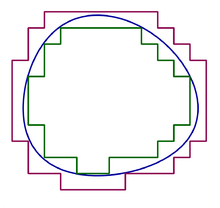
\includegraphics[scale=0.7]{../images/jordan_wiki.png}
 	\caption{Aproximação interior e exterior por conjuntos elementares}
 	\label{jordanwiki}
 \end{figure}

A referência \cite{math3} formaliza explicitamente sequência específicas de conjuntos elementares para que o ínfimo e supremo da definição \ref{inner_outer} não sejam tomados sobre todos os conjuntos elementares possíveis, e sim, em uma escolha particular deles.

Não iremos reproduzir a formalização aqui, mas a noção intuitiva para construção é particionar o $\rn$ em caixas formadas pelos grid $\mathbb{Z}^n$. Se $S$ é nosso conjunto, a aproximação interior será formada pelas caixas inteiramente contidas em $S$, e a aproximação exterior, por todas aquelas que possuem interseção não vazia com S. Após isso, particiona-se cada lado do grid pela pela metade, criando-se caixas geradas por $\frac12\mathbb{Z}^n$, e redefinindo quem são as caixas interiores e exteriores. Repedindo esse processo, com o grid $\frac{1}{2^k}\mathbb{Z}^n$ variando $k$ nos naturais, teremos uma sequência de conjuntos elementares contida em $S$ e outra contendo $S$. A Figura \ref{inner_jordan} extraída de \cite{princeton} ilustra dois passos do processo de aproximação interior de um conjunto aberto $\mathcal{O}\subset\rr$.

\begin{figure}[!htb]
	\centering
	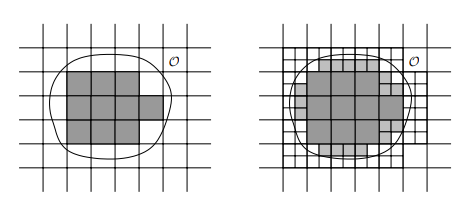
\includegraphics[scale=0.95]{../images/inner_jordan.png}
	\caption{Aproximação Elementar Interior de Jordan}
	\label{inner_jordan}
\end{figure}

\subsection{Conjuntos Jordan Mensuráveis}
Finalmente vamos estabelecer o conceito de mensurabilidade que restringirá os tipos de conjuntos que iremos considerar como domínio de parametrizações depois.

\begin{defi}
	Um conjunto $S\subseteq\rn$ é dito \textbf{Jordan mensurável} ou \textbf{J-mensurável} quando a medida exterior de Jordan coincide com a medida interior, isto é,
	$$\mu_{*}(S)=\mu^{*}(S)$$
	O valor comum é denotado\footnote{Na seção seguinte usamos a mesma notação $\mu$ para representar outra coisa} por $\mu(S)$ e chamado de \textbf{Medida de Jordan} de $S$.
\end{defi}

	Um exemplo de conjunto não mensurável à Jordan é $S=\mathbb{Q}\cap[0,1]$ como subconjunto de $\real$.
	Qualquer cobertura superior desse conjunto por conjuntos elementares (uniões finitas de intervalos), precisa cobrir $[0,1]$ inteiramente, sendo assim $\mu^{*}(S)\geq1$. Para provar que $\mu^{*}(S)=1$ podemos tomar a sequência decrescente $[0,1+\frac1/n]$ cujo ínfimo da medida será 1.
	Entretanto $\mu_{*}(S)=0$ por vacuidade de conjuntos elementares interiores. De fato não é possível definir um intervalo em $\mathbb{Q}\cap[0,1])$ que esteja inteiramente contido $S$, pela densidade dos irracionais. Sendo assim o supremo de $\mu_{*}$ estaria sendo tomado sobre o conjunto vazio que tem medida zero.
	
	Com argumentos análogos é possível provar que $\mu_{*}(\mathbb{Q}^n\cap[0,1]^n)=0$ e $\mu^{*}(\mathbb{Q}^n\cap[0,1]^n)=1$
	
	Um critério para checar se um conjunto limitado $S\subset \rn$ é verificar se a função 
	
	$$\one_S(x)=\begin{cases}1,\text{ se }x\in S\\0,\text{ se }x \notin S\end{cases}$$
	
	é integrável à Riemann, ou seja, a integral 
	
	$$\Int_Sdx_1\ldots dx_n$$
	
	está bem definida. A demonstração formal é consequência direta do Teorema 5 do artigo \cite{frink}, que trás uma abordagem mais geral e bem interessante interessante sobre condições de integrabilidade de funções limitadas.  
	
	
\section{Primeira Forma Fundamental}
	\label{fff}
	\subsection{Definições Iniciais}
	\begin{defi}
		 \textbf{(Superfície Regular)\cite{ronaldo}} Um conjunto $S\subset\real^3$ é uma superfície regular, quando $\forall p\in S$, existem $U\subset\rr$ aberto, $W\subset\real^3$ aberto contento $p$ e um difeomorfismo 
		$$\sigma:U\to W\cap S.$$
	A aplicação acima é chamada de parametrização local de $S$ em $p$.
	\end{defi}
	
	\begin{defi}
		\textbf{(Primeira Forma Fundamental)\cite{ronaldo}} Dada uma superfície regular $S$ e um ponto $p\in S$, definimos a Primeira Forma Fundamental de $S$ em $p$ como o produto escalar de $\real^3$ restrito ao plano tangente de $S$ em $p$, $T_pS$:
		\begin{align*}
			I_p:T_pS&\to\real\\
			w&\mapsto \langle w,w\rangle=||w||^2
		\end{align*}
	\end{defi}

	Se $\sigma:U\subset\rr\to\sigma(U)\subset S$ é uma parametrização, dizemos que as funções:
	\begin{align*}
		E(u,v)&=\langle \sigma_u(u,v),\sigma_u(u,v)\rangle\\
		F(u,v)&=\langle \sigma_u(u,v),\sigma_v(u,v)\rangle\\
		G(u,v)&=\langle\sigma_v(u,v),\sigma_v(u,v)\rangle
	\end{align*}
	são chamadas de coeficientes da primeira forma fundamental de $S$ em relação à $\sigma$. A justificativa para esse nome segue do formato da expressão de $I_{\sigma(u,v)}$; Dado um $w\in T_pS$ qualquer, podemos escrevê-lo na base das derivadas parciais como $w=a\sigma_u(u,v)+b\sigma_v(u,v)$. Assim:
	\begin{align*}
		I_{\sigma(u,v)}&=\langle a\sigma_u+b\sigma_v,a\sigma_u+b\sigma_v\rangle\\
		&=a^2\langle\sigma_u,\sigma_u\rangle+2ab\langle\sigma_u,\sigma_v\rangle+b^2\langle\sigma_v,\sigma_v\rangle\\
		&=a^2E(u,v)+2abF(u,v)+b^2G(u,v)
	\end{align*}

	Dessa forma podemos expressar a primeira formal fundamental como a forma quadrática $I_{\sigma(u,v)}(w)=w^TAw$, onde 
	$$A=\begin{bmatrix}
		E(u,v)&F(u,v)\\
		F(u,v)&G(u,v)
	\end{bmatrix}$$
	
	Vamos enunciar agora uma proposição que será usada na justificativa da fórmula de área:
	
	\begin{proposition}
		\label{prop1}
		Dada uma superfície regular $S$, para todo $p_0\in S$, existe um aberto $V\subset S$ que contém $p_0$ e é o gráfico de uma função diferenciável definida em um aberto do plano $T_{p_0}S+p_0$.
	\end{proposition}
	 A demonstração será omitida, pode ser encontrada na página 53 de \cite{ronaldo}.
	\subsection{O Cálculo de Áreas}
		Pela seção \ref{jordan}, concluímos que um conjunto $\Omega\subset\rr$ é \textit{J-mensurável} quando a função característica $\one_\Omega$ é integrável, ou seja,
		$$\displaystyle\int_\Omega dudv$$
		está bem definida no sentido de Riemann, e é a área de $\Omega$, que detonaremos por $\mu(\Omega)$.
		
		Dada uma superfície regular $S$ e uma parametrização $\sigma:U\subset\rr\to \sigma(U)\subset S$. Dado $\rcur\subset \sigma(U)$, se $\sigma^{-1}(\rcur)$ for limitado e J-mensurável em $\rr$, então diremos que $\rcur$ é J-mensurável. Assim, definimos a área de $\rcur$ como:
		$$\mu(\rcur)=\displaystyle\int_{\sigma^{-1}(\rcur)}||\sigma_u\times\sigma_v||dudv$$
		
		Para chegar nessa fórmula construtivamente, definamos um quadrado $Q=I\times I\subset\rr$ que contem $\Omega=\sigma^{-1}(\rcur)$. Tomando $\mathscr{P}=\{K_1,\ldots,K_n\}$ uma partição de $Q$ formada por retângulos de lados paralelos aos eixos coordenados, defina $|\mathcal{P}|:=\max\{|\text{diag}(K_i)|;k=1,\ldots,n\}$, onde $|\text{diag}(K_i)|$ é comprimento da diagonal do retângulo $K_i$.
	
		Para cada $K_i$, escolha um ponto $a_i\in\op{int}(K_i)\cap \Omega$. Pela Proposição \ref{prop1}, em uma vizinhança de $p_i=\sigma(a_i)$, $S$ é gráfico de uma função diferenciável de domínio em um aberto do plano $T_{p_i}S+p_i$. Além disso, a derivada direcional
		
		\begin{align*}
			d\sigma_{a_i}:\rr\to& T_{p_i}S\\
				w=(w_1,w_2)\mapsto& \langle\nabla\sigma_{a_i},v\rangle\\
				=&\sigma_u(a_i)w_1 + \sigma_v(a_i)w_2
		\end{align*} 
		
		é um operador que leva o retângulo $K_i$ em um paralelogramo $P_i\subset T_{p_i}S$ tal que $p_i$ pertence ao interior de $P_i'=P_i+p_i$. Assim $\sigma(K_i\cap\Omega)$ de $\rcur$ será uma boa aproximação de $P_i'$ conforme a diagonal de $K_i$ tender a zero. A figura \ref{fig1} ilustra o processo da aplicação de $\sigma$ à partição, e depois, o difeomorfismo local entre $P_i'$ e a superfície, tal figura foi extraída da referência \cite{ronaldo}, que usa a notação $X$ para nosso $\sigma$. 
		
		\begin{figure}[!htb]
			\centering
			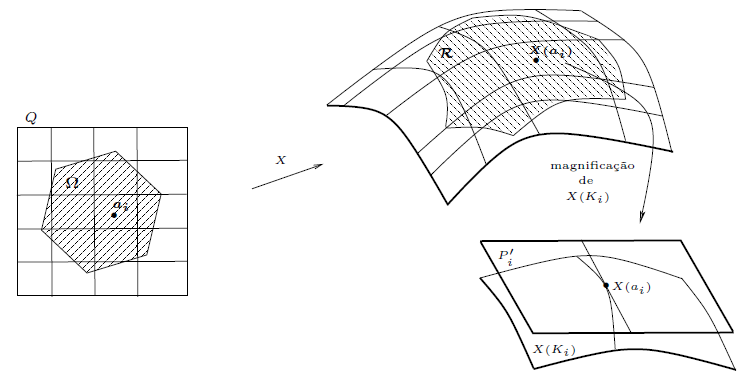
\includegraphics[scale=0.7]{../images/fff_fig1.png}
			\label{fig1}
			\caption{Aproximação tangente}
		\end{figure}
	
		Veja que $\rcur=\displaystyle\bigcup_{i=1}^n\sigma(K_i\cap\Omega)$. Assim definimos a área de $\rcur$ como:
		\begin{align}
			\displaystyle\lim_{|\mathscr{P}|\to0}\sum_{i=1}^n\mu(P_i)\label{lim}
		\end{align}
		Com $\mathscr{P}$ variando sobre o conjunto de todas as partições de $Q$. Se $I=[a,b]$, e $Q=I\times I$ poderíamos tomar em particular a partição produto que subdivide $i$ em $n$ intervalos iguais de tamanha $(b-a)/n$. Sendo assim teríamos $n^2$ retângulos ao invés de $n$, mas as definições acima permaneceriam consistentes. O limite \ref{lim} poderia então poderia ser tomado neste caso com $n\to\infty$, já que a diagonal de cada retângulo $K_i$ (quadrado no caso) dessa partição é por Pitágoras $\frac{(b-a)\sqrt2}n$. Assim $n\to\infty$ implicaria $|\mathscr{P}|=\frac{(b-a)\sqrt2}n\to 0$. Teríamos nesse caso em particular:
		\begin{align*}
			\displaystyle\lim_{n\to\infty}\sum_{i=1}^{n^2}\mu(P_i)
		\end{align*}
	
	 Se $K_i$ tem lados medindo $t_i$ e $s_i$ de tal forma que tais lados sejam translações de $t_ie_1$ e $s_ie_2$ com $e_1,e_2$ canônicos de $\rr$, então os lados de $P_i=d\sigma_{a_i}(K_i)$ são translações de:
	 \begin{align*}
	 	d\sigma_{a_i}(t_ie_1)&=t_i\sigma_u(a_i)\cdot1+t_i\sigma_v(a_i)\cdot0=t_i\sigma_u(a_i)\\
	 	d\sigma_{a_i}(s_ie_2)&=s_i\sigma_u(a_i)\cdot0+s_i\sigma_v(a_i)\cdot1=s_i\sigma_v(a_i)
	 \end{align*}
 
 	De resultados de Geometria Analítica, temos que a área do paralelogramo é a norma do produto vetorial dos dois vetores que o definem, assim:
 	
 	\begin{align*}\mu(P_i)&=||d\sigma_{a_i}(t_ie_1)\times d\sigma_{a_i}(s_ie_2)||\\
 		&=||t_i\sigma_u(a_i)\times s_i\sigma_v(a_i)||\\
 		&=s_it_i||\sigma_u(a_i)\times\sigma_v(a_i)||\\
 		&=\mu(K_i)||\sigma_u(a_i)\times\sigma_v(a_i)||
 	\end{align*}
 
 Com isso, o limite em \ref{lim} será:
 $$\displaystyle\lim_{\mathscr{P}\to0}\sum_{i=1}^n\mu(K_i)||\sigma_u(a_i)\times\sigma_v(a_i)||$$
 que é por definição, a integral de Riemann da função $f(u,v)=||\sigma_u(u,v)\times\sigma_v(u,v)||$ no conjunto $\Omega=\sigma^{-1}(\rcur)$. Assim fica justificada a fórmula:
 
 \begin{align*}
 	\mu(\rcur)=\displaystyle\int_{\Omega}||\sigma_u(u,v)\times\sigma_v(u,v)||dudv
 \end{align*}

Vamos agora encontrar uma expressão para a área em termos da Primeira Forma Fundamental.

Usando sem provar que dados $a,b$ vetores com ângulo $\theta$ entre eles vale $||a\times b||=||a||\cdot||b||\sin\theta$, e $\cos\theta=\dfrac{\langle a,b\rangle}{||a||\cdot||b||}$, temos\footnote{OBS: Omitimos as entradas $(u,v)$ das notações de $\sigma_u,\sigma_v,E,F$ e $G$ para não sobrecarregar a notação.}:

\begin{align*}
	||\sigma_u(u,v)\times\sigma_v(u,v)||^2&=||\sigma_u||^2||\sigma_v||^2\sin^2\theta\\&=||\sigma_u||^2||\sigma_v||^2(1-\cos^2\theta)\\
	&=||\sigma_u||^2||\sigma_v||^2\left(1-\dfrac{\langle\sigma_u,\sigma_v\rangle^2}{||\sigma_u||^2||\sigma_v||^2}\right)\\
	&=||\sigma_u||^2||\sigma_v||^2-\langle\sigma_u,\sigma_v\rangle^2
\end{align*}

Substituindo $E=||\sigma_u||^2$, $F=\langle\sigma_u,\sigma_v\rangle$ e $G=||\sigma_v||^2$, temos:

$$||\sigma_u(u,v)\times\sigma_v(u,v)||=\sqrt{EG-F^2}$$

E com isso, finalmente, estabelecemos a belíssima fórmula do cálculo de área em superfícies via Primeira Formal Fundamental:

\begin{align}
	\displaystyle\mu(\rcur)=\int_{\sigma^{-1}(\rcur)}\sqrt{EG-F^2}dudv \label{theformula}
\end{align}

\subsection{Exemplo: Superfícies de Revolução}

 Seja $S$ uma superfície de revolução cuja curva geratriz admite parametrização \textit{unit-speed} contida no plano $XZ$ por exemplo, dada por:
\begin{align*}
	\alpha:I\subset\real&\to S\\
	v &\mapsto (x(v),0,z(v)),
\end{align*}
com $x(v)>0,~\forall v \in I$
 Girando essa curva sobre o eixo coordenado $z$ podemos parametrizar a superfície cobrindo-a quase completamente, através de:
  \begin{align*}
  	\sigma:U&\to S\\
  	(u,v)&\mapsto (x(v)\cos u,x(v)\sin u,z(v)),
  \end{align*}
com $U=(-\pi,\pi)\times I$.

Calculando as derivadas parciais, temos:
\begin{align*}
	\sigma_u(u,v)&=(-x(v)\sin u,x(v)\cos u,0)\\
	\sigma_v(u,v)&=(x'(v)\cos u,x'(v)\sin u,z'(v))
\end{align*}
Os coeficientes da Primeira Forma Fundamental serão então:
\begin{align*}
	E(u,v)&=||\sigma_u(u,v)||^2=(x(v))^2(\sin^2u+\cos^2u)\\&=(x(v))^2\\
	F(u,v)&=\langle\sigma_u,\sigma_v\rangle=\cos u\sin u(-x(v)x'(v)+x(v)x'(v))\\&=0\\
	G(u,v)&=||\sigma_v(u,v)||^2=(x'(v))^2(\cos^u+\sin^2u)+(z'(v))^2=(x'(v))^2+(z'(v))^2\\&=||\alpha'(v)||=1
\end{align*}

Tomando $a,b\in I$ com $a<b$, a área de $\rcur=\sigma(\Omega)$ com $\Omega=(-\pi,\pi)\times[a,b]\subset U$, pode ser calculada diretamente pela fórmula \ref{theformula}. A justificativa de $\rcur$ ser J-mensurável, é que $\Omega$ é claramente limitado. Uma aproximação interior de Jordan pode ser $A_n=[-\pi+\frac1n,\pi-\frac1n]\times[a+\frac1n,b-\frac1n]$ que é caixa segundo a Definição \ref{box}, de medida $m(A_n)=(2\pi-\frac2n)\cdot((b-a)-\frac2n)$. Uma aproximação exterior via caixas poderia ser $B_n=[-\pi-\frac1n,\pi+\frac1n]\times[a-\frac1n,b+\frac1n]$, com $m(B_n)=(2\pi+\frac2n)\cdot((b-a)+\frac2n)$. 

Com $(m(A_n))_{n\in\mathbb{N}}$ sendo sequencia crescente e $(m(B_n))_{n\in\mathbb{N}}$ decrescente, ambas limitadas, podemos trocar supremo e ínfimo por limite, obtendo a igualdade da medida interior e exterior de Jordan.
\begin{align*}
	\mu_*(\Omega)&=\sup\{m(A_n);n\in\mathbb{N}\}=\lim_{n\to\infty}m(A_n)\\
	&=\lim_{n\to\infty}(2\pi-2/n)\cdot((b-a)-2/n)\\
	&=2\pi(b-a)\\
	\mu^{*}(\Omega)&=\inf\{m(B_n);n\in\mathbb{N}\}=\lim_{n\to\infty}m(B_n)\\
	&=\lim_{n\to\infty}(2\pi+2/n)\cdot((b-a)+2/n)\\
		&=2\pi(b-a)
\end{align*}

Poderíamos utilizar também o critério de Riemman, e facilmente concluiríamos a J-mensurabilidade de $\Omega$ constatando que $\Int_{(\pi,\pi)\times[a,b]}dudv$ existe e é igual a $2\pi(b-a)$.

Estando justificada a Jordan-mensurabilidade de $\Omega$, segue o cálculo da área:

\begin{align}
	\mu(\rcur)&=\Int_{\Omega}\sqrt{EG-F^2}dudv\nonumber\\
	&=\Int_a^b\Int_{-\pi}^{\pi}\sqrt{(x(v))^2\cdot1-0^2}dudv\nonumber\\
	&=\Int_a^b\Int_{-\pi}^{\pi}|(x(v))|dudv\nonumber\\
	&=\Int_a^b\Int_{-\pi}^{\pi}(x(v))dudv\label{abs}\\
	&=2\pi\Int_a^bx(v)dv\nonumber
\end{align}
Na qual a passagem \ref{abs} se justifica pois assumimos $x(v)>0$. este resultado é conhecido como Teorema de Pappus.

No caso de um cilindro gerado pela reta no plano $XZ$, $\alpha(v)=(r,0,v)$ com $r$ fixo como raio do cilindro, como $||\alpha'(v)||=1$ aplicar Pappus diretamente sem reparametrização. Considerando a região de entre $a$ e $b$ obtemos: $2\pi\int_a^ b rdv=2\pi r(b-a)$.
	\begin{appendices}
		\section{Demonstrações Seção 2}
		\label{appA}
			\subsection{Proposição 1 - Decomposição por caixas quase disjuntas}
			Relembrando o enunciado da Proposição \ref{elementary}:
			
			Para todo conjunto elementar $B\subseteq\rn$, existem caixas duas a duas quase disjuntas $B_1',\ldots,B_m'$ tais que $B=B_1'\cup\ldots\cup B_m'$.
			
			Este resultado é um caso particular do exercício 10.D do Bartle\cite{bartle2014elements}:
			
			\textbf{Exercício 10.D (Bartle):} Sejam $(X,\bd X)$ e $(Y,\bd Y)$ espaços mensuráveis. Se $A_j\in\bd X$ e $B_j\in\bd Y$ para $J=1,\ldots,m$, então o conjunto 
			$$\bigcup_{j=1}^{m}(A_j\times B_j)$$
			pode ser escrito como união finita disjunta de retângulos em $Z=X\times Y$.
			
			onde $\bd X,\bd Y$ são as $\sigma$-álgebras geradas por $X$ e $Y$ respectivamente, e \textit{retângulo} para o Bartle é um produto $A\times B$ com $A\in\in\bd X,B\in\bd Y$. A demonstração desse exercício será omitida, ela pode ser feita puramente via teoria dos conjuntos e a noção de produto cartesiano, provando que um conjunto está contido no outro e vice-versa  para concluir a igualdade.
			
			Nossa proposição é consequência desse exercício, pois o caso $X=Y=\real$, com $\bd X=\bd Y=\mathcal{B}$ borelianos da reta provaria a proposição para retângulos em $\rr$. A única atenção seria em forçar que a união finita de retângulos garantida pelo exercício sejam fechados e quase disjuntos. A extensão para o $\rn$, segue considerando $(X,\bd X)=(\real^{n-1},\mathcal{B}(\real^{n-1}))$ e $(Y,\bd Y)=(\real,\mathcal{B})$, onde $\mathcal{B}(\real^{n-1})$ é a $\sigma$-álgebra de Borel gerada por $\rn$. A existência de tal espaço de medida pode ser construída indutivamente duas a duas usando os resultados do Capítulo 10 do Bartle\cite{bartle2014elements} para formalização de medidas produtos. Podemos argumentar que um retângulo de $(\real^{n-1}\times\real)$ no sentido do Bartle pode ser transformada em uma caixa de $\rn$ no sentido da definição \ref{box} simplesmente adicionando bordas nos intervalos intrínsecos, o que poderia quebrar a disjunção, mas não quebra a quase-disjunção.
			
			Entrando na demonstração do exercício, vamos provar apenas o caso onde $A_j\subset X$ e $B_j\subset Y$ que já basta para nossa Proposição, mas o resultado vale para conjuntos quaisquer das $\sigma$-álgebras.
			
			Os resultados são gerais mas podemos pensar $A_j,B_j$ como intervalos fechados da reta. De fato vamos apelar para essa simplificação para geração de caixas quase disjuntas no final. 
			
			Defina $R_j=A_j\times B_j$ e $F_1=R_1$, $F_2=R_2\backslash R_1,\ldots, F_k=R_k\backslash\bigcup_{j=1}^{k-1}R_j$.
			
			Por construção $\displaystyle\bigcup_{j=1}^{m}F_j=\bigcup_{j=1}^{m}R_j$ e os $F_i$'s são disjuntos. Se provarmos que cada $F_i$ é um retângulo ou pelo menos uma união finita de retângulos disjuntos, o exercício fica provado, pois para $i\neq j$, $F_i\cap F_j=\emptyset$.
			
			$F_1$ é obviamente retângulo. Pelo primeiro ponto do Exercício 10.E do Bartle\cite{bartle2014elements} temos que $F_2=R_2\backslash R_1$ pode ser expresso como união finita (disjunta) de retângulos:
			
			\textbf{Exercício 10.E (Bartle):} Subtração de retângulos da $\sigma$-álgebra é uma união disjunta de dois retângulos da $\sigma$-álgebra, isto é:
			Sejam $A_j\subseteq X$ e $B_j\subseteq Y$, $j=1,2$. Então
			\begin{itemize}
				\item $(A_1\times B_1)\backslash(A_2\times B_2)=[(A_1\cap A_2)\times (B_1\backslash B_2)]\cup[(A_1\backslash A_2)\times B_1]$
				\item $(A_1\times B_1)\cap(A_2\times B_2)=(A_1\cap A_2)\times(B_1\cap B_2)$
			\end{itemize}
			
			Como $(A_1\cap A_2)\times (B_1\backslash B_2)$ e $(A_1\backslash A_2)\times B_1$ são retângulos no sentido de serem produtos entre elementos das $\sigma$-álgebras $\bd X,\bd Y$ a afirmação acima sobre $F_2$ é válida.
			
			Temos então que para $m=2$, $\bigcup_{j=1}^{m}R_j$ pode ser expresso como união finita de retângulos disjuntos.
			
			Por indução finita, suponha que para algum $m$ temos $\bigcup_{j=1}^{m}F_j=\bigcup_{j=1}^{m}R_j$ possa ser expresso como união finita disjunta de retângulos $D=\bigcup_{\ell=1}^{M} D_{\ell}$, com $D_{\ell}$ retângulos disjuntos dois a dois.
			
			Tome $D\cup R_{m+1}$ e o escreva como a união disjunta $R_{m+1}\cup(D\backslash R_{m+1})$, Assim
			\begin{align*}
				\bigcup_{j=1}^{m+1}R_j&=R_{m+1}\cup(D\backslash R_{m+1})\\
				&=R_{m+1}\cup\left(\bigcup_{\ell=1}^{M} D_{\ell}\backslash R_{m+1}\right)\\
				&=R_{m+1}\cup\left(\bigcup_{\ell=1}^{M} (D_{\ell}\backslash R_{m+1})\right)
			\end{align*}
		Como a subtração de retângulos $D_{\ell}\backslash R_{m+1}$ pode ser expressa como união finita de retângulos disjuntos, então a união sobre $\ell$ será uma união de retângulos disjuntos e consequentemente $R_{m+1}\cup\left(\bigcup_{\ell=1}^{M} (D_{\ell}\backslash R_{m+1})\right)$ também será. Portanto conclui-se o passo indutivo.
		
		\subsection{A Fórmula da Discretização}
			Dada uma caixa $B\subseteq \rn$, vale que 
			
			$$m(B)=\lim_{k\to\infty}\dfrac{1}{k^n}\#(B\cap\frac1k\mathbb{Z}^n)$$
			
			na qual $\frac1k\mathbb{Z}^n=\{(\frac{a_1}k,\ldots,\frac{a_n}k);a_1,\ldots,a_n\in\mathbb{Z}\}$ e $\#$ representa cardinalidade.
			
			Esta fórmula será usada na demonstração da Proposição \ref{elementary_masure}.
			
			\textbf{Demonstração da Fórmula:} Tome o caso onde $B$ é um intervalo $[a,b]$. Assim,
			
			\begin{align*}
				\#(B\cap\frac1k\mathbb{Z})&=\#\{z\in\mathbb{Z};\frac z k\in B\}\\
				&\leq\{z\in\mathbb{Z};ka\leq z \leq kb\}\\
				&\leq \{z\in\mathbb{Z};\lfloor ka \rfloor\leq z \leq \lceil kb \rceil\}\\
				&= \lceil kb \rceil-\lfloor ka \rfloor+1\\
				&\leq (kb+1)-(ka-1)+1\\
				&=k(b-a)+3
			\end{align*}
		
		Analogamente:
		
		\begin{align*}
				\#(B\cap\frac1k\mathbb{Z})&\geq\{z\in\mathbb{Z};ka< z < kb\}\\
				&\geq\{z\in\mathbb{Z};\lceil ka\rceil < z < \lfloor kb\rfloor\}\\
				&=\lfloor kb\rfloor-\lceil ka\rceil+1\\
				&\geq(kb-1)-(ka+1)+1\\
				&=k(b-a)-1-1+1\\
				&=k(b-a)-1
		\end{align*}
		
		Dividindo por $k$ temos $(b-a)-\frac1k\leq\frac1k\#(B\cap\frac1k\mathbb{Z})\leq (b-a)+\frac3k$. Pela "Regra so Sanduíche", quando $k\to \infty$, $\frac1k\#(B\cap\frac1k\mathbb{Z})\to(b-a)=m(B)$. O que prova o resultado para intervalos.
		
		Tomemos agora $B=I_1\times\ldots\times I_n$, com $I_1,\ldots,I_n$ intervalos fechados $I_k=[a_j,b_j]$, $a_j<b_j$. Dessa forma
			$$B\cap\frac1k\mathbb{Z}^n=\left(I_1\cap\frac1k\mathbb{Z}\right)\times\ldots\times\left(I_n\cap\frac1k\mathbb{Z}\right),$$
			
			o que implica:
			
			$$\displaystyle\#\left(B\cap\frac1k\mathbb{Z}^n\right)=\prod_{j=1}^n\#\left(I_j\cap\frac1k\mathbb{Z}\right)$$
			\end{appendices}
	
	Dividindo ambos os lados por $k^n$ e utilizando o resultado já conhecido de intervalos, temos:
	\begin{align*}
		&\dfrac{1}{k^n}\#\left(B\cap\frac1k\mathbb{Z}^n\right)=\dfrac{1}{k^n}\prod_{j=1}^n\#\left(I_j\cap\frac1k\mathbb{Z}\right)\\
		&\Rightarrow \dfrac{1}{k^n}\#\left(B\cap\frac1k\mathbb{Z}^n\right)=\prod_{j=1}^n\dfrac1k\#\left(I_j\cap\frac1k\mathbb{Z}\right)\\
		&\Rightarrow\lim_{k\to\infty}\dfrac{1}{k^n}\#\left(B\cap\frac1k\mathbb{Z}^n\right)=\lim_{k\to\infty}\prod_{j=1}^n\dfrac1k\#\left(I_j\cap\frac1k\mathbb{Z}\right)\\
		&=\prod_{j=1}^n\lim_{k\to\infty}\dfrac1k\#\left(I_j\cap\frac1k\mathbb{Z}\right)\\
		&=\prod_{j=1}^n(b_j-a_j)\\
		&=m(B)
	\end{align*}

	Como queríamos demonstrar.
	
	\subsection{Proposição 2 - Medida de Conjuntos elementares}
	
	Para provar a Proposição \ref{elementary_masure}, note que pelo menos uma decomposição por caixas quase disjuntas existe pela Proposição \ref{elementary}. Tome então uma decomposição arbitrária $B_1',\ldots,B_m'$ dois a dois quase disjuntos, tal que $B=B_1'\cup\ldots\cup B_m'$. 
	
	Utilizando a Fórmula da Discretização, temos:
	
	\begin{align*}
		\displaystyle\sum_{i=1}^{m}m(B_i')&=\sum_{i=1}^m\lim_{k\to\infty}\frac1{k^n}\#\left(B_i'\cap\frac1k\mathbb{Z}^n\right)\\
		&=\lim_{k\to\infty}\dfrac{1}{k^n}\sum_{i=1}^{m}\#\left(B_i\cap\frac1k\mathbb{Z}^n\right)\\
		&=\lim_{k\to\infty}\frac{1}{k^n}\left(\bigcup_{i=1}^m B_i'\cap\dfrac1k\mathbb{Z}^n\right)\\
		&=\lim_{k\to\infty}\frac{1}{k^n}\#\left(B\cap\frac1k\mathbb{Z}^n\right)
	\end{align*}

	que é justamente a fórmula de discretização para $m(B)$, o que finaliza a demonstração já que a decomposição $B_1',\ldots,B_m'$ foi tomada como arbitrária.
	
	\newpage
	\addcontentsline{toc}{section}{Referências}
	%	\bibliography{refs}
	\printbibliography
\end{document}